\documentclass[12pt]{article}
\usepackage[czech]{babel}
\usepackage[utf8]{inputenc}
\usepackage[IL2]{fontenc}
\usepackage{wrapfig}
\usepackage{graphicx}
\usepackage{scrextend}
\usepackage{cprotect}
\usepackage{float}
\usepackage{hyperref}
\usepackage{indentfirst}
\newcommand{\htmltag}[1]{%
	\scalebox{.6}[1]{$<$}{\ttfamily#1}\scalebox{.6}[1]{$>$}%
}

\begin{document}
\pagenumbering{gobble} %bez cisel
\begin{titlepage}
\centerline{
\includegraphics[width=10cm]{img/logo.jpg}}
\begin{center}
\vspace{30px}
{\Huge
\textbf{Semestrální práce KIV/PC}\\
\vspace{1cm}
}
{\Large
\textbf{Řešení kolizí frekvencí sítě vysílačů}\\
}
\vspace{1cm}
{\large
Pavel Třeštík\\
}
{\normalsize
A17B0380P
}
\end{center}
\vspace{\fill}
\hfill
\begin{minipage}[t]{7cm}
\flushright
\today
\end{minipage}
\end{titlepage}

\tableofcontents
\newpage
\pagenumbering{arabic} %
% Zadání
%
\section{Zadání}
%
Naprogramujte v ANSI C přenositelnou konzolovou aplikaci, která jako vstup
načte z parametru příkazové řádky název textového souboru obsahující
informace o parametrech a pozicích vysílačů na mapě a na jeho základě
přidělí každému vysílači frekvenci tak, abz jeho signál nerušil
vysílání vysílačů v jeho bezprostředním okolí.\\

Program se bude spouštět příkazem \texttt{freq.exe <filename>}. Symbol
\texttt{<filename>} zastupuje jméno textového souboru, který obsahuje
informace o rozmístění vysílačů na mapě a o dostupných vysílacích
frekvencích, které jim je možné přidělit.\\

Výsledkem práce programu bude výpis do konzole, na kterém bude seznam
přidělených frekvencí každému vysílači ze vstupního souboru. V případě
chyby nebo neřešitelné situace nechť program skončí výpisem příslušné
chybové hlášky (v angličtině).\\

Pokud nebude na příkazové řádce uvede přávě jeden argument, vypište chybové
hlášení a stručný návod k použití programu v angličtině podle běžných 
zvyklostí. Vstupem programu je pouze argument na příkazové řádce - interakce
s uživatelem pomocí klávesnice či myši v průběhu práce programu se neočekává.\\

Zadání ve své kompletní podobě najdete na: \url{https://www.kiv.zcu.cz/
studies/predmety/pc/doc/work/sw2019-02.pdf}\\
%
% Analýza problému
%
\pagebreak
%
\section{Analýza problému}
%
Tato úloha načte informace ze souboru. Poté s těmito informacemi provede svou 
funkčnost a vypíše výsledek na konzoli. Aby toto bylo možné je nutné zvolit
vhodný způsob uložení načtených informací do paměti. Načítají se 3 infromace: 
frekvence, vysílače a rádius. Rádius je pouze jedno celé číslo, takže není 
třeba se jím zabývat. Výsílače a frekvence se ale skládají z více informací 
a neznámého počtu, proto je třeba vybrat vhodný způsob ukládání struktur.\\

Po té program potřebuje zjistit sousedící vysílače a následně jim přiřadit 
dostupné frekvence. K tomu je třeba uchovat sousedy každého vysílače.
Dále je v zadání doporučeno použít datovou strukturu zásobník, proto zde bude
také popsána.
%
\subsection{Způsoby uložení vysílačů a frekvencí}
%
Možné způsoby jsou pole, dynamické pole (rozšiřující se podle potřeby), linked 
list či nějáká jeho obdoba.\\

\textbf{Pole} - výhodami jsou: nízká paměťová náročnost a konstantní přístup
k prvku pomocí indexu, pokud index známe. Nevýhodou je, že předem musí být 
znám počet prvků, tudíž by bylo nutné nejdřív soubor projít a spočítat počty 
frekvencí a vysílačů, což by se o velkých souborů mohlo projevit jako časově 
náročnější a potenciálně nebezpečný (při nečekaném ukončení programu).\\

\textbf{Dynamické pole} - oproti poli má výhodu, že není předem nutné znát 
počet načítaných prvků. Ovšem tato výhoda je omezena nevýhodou v podobě 
paměťové náročnosti. Rozšiřovat pole pouze o malý počet prvků by bylo 
časově i výpočetně náročné a rozšiřovat ho o například polovinu by mohlo 
způsobit alokování velkého bloku paměti, který se nemusí vůbec využít.\\

\textbf{Linked list} - výhodou je, že není třeba znát počet prvků a 
pravděpodobně je paměťově efektivnější než dynamické pole. Kromě dat struktur 
uchovává akorát pointer na další prvek. Nevýhodou je přídávání, které v 
klasickém linked listu musí dojít na konec listu a vložit nový prvek. Tato 
nevýhoda může být ale snadně odstraněna.
%
\subsection{Uchování sousedů}
%
Sousedi mohou být zaneseni do matice sousednosti či uchováváni jako některá z 
datových struktur použitých k uložení vysílačů a frekvencí. Obě řešení 
zaberou paměť navíc, ovšem matice bude zabírat více paměti, protože uchovává 
sousednost každého bodu s každým, proto uchovává spoustu neužitečných dat. 
Oproti tomu ukládat sousedy do pole, linked listu či jiné zvolené struktury 
bude pouze uchovávat pointery na sousedy a pokud vysílač nemá sousedy nebude 
zabírat žádnou paměť. Výpočetně se jedná o zhruba stejně složité úlohy, protože
je nutné zjistit všechny sousedy každého bodu tím, že je nutné porovnat pozice
každého vysílače o proti všem ostatním a tudíž žádné řešení není významně lepší
po výpočetní stránce.
%
\subsection{Zásobník}
%
Dá se považovat za druh linked listu. Prvek je vkládán na první pozici listu a 
poslední přidaný (první v listu) je vyjímán. Toto zajišťuje, že prvky jsou 
vyjímány v opačném pořadí v jakém byly vloženy (první vložen bude vyjmut 
poslední).
%
% Implementace
%
\section{Implementace}
%
\subsection{Struktura projektu}
%
%TODO: obrazek\\ popis?
%
\subsection{Použité struktury}
%
Pro uchování frekvencí a vysílačů je použita upravená struktura linked list.
Jak je zmíněno v analýze úlohy, tato struktura poskytuje jednoduchou
rozšiřitelnost za cenu paměti uchovávájící pointer na další prvek. Struktura
je vylepšená tím, že během vytváření listu frekvencí/ vysílačů se uchovává 
pointer na poslední prvek, tudíž není třeba procházet celý list pro přidání
prvku.\\

Pro sousedy vysílačů je také použita struktura linked list, ovšem zde už není 
uchováván poslední prvek, tudíž při přidání prvku se musí projít celý linked
list.\\

V programu je také použita struktura stack. Tato struktura je již popsána v 
analýze úlohy a její využítí bude zmíněno v následující sekci.
%
\subsection{Použité řešení}
%
Pro nalezení sousedů jednotlivých vysílačů se porovnává pozice procházeného
vysílače proti pozicím všech vysílačů, které se nachází v linked listu od 
pořadí procházeného vysílače dál. V případě, že vysílače jsou sousedé, přidají
se navzájem do svých respektivních listů sousedů. Postup je znázorněn na
Obrázku\\ 
%TODO: obrazek\\

Po nalezení všech sousedů každého vysílače se začnou přiřazovat frekvence
jednotlivým vysílačům (obravování grafu). Pro tuto část je použit algoritmus
uvedený v zadání. Zjednodušeně: v linked listu se vybere první vysílač. Pokud 
nemá dosud přiřazenou frekvenci, je přidán do stacku. Pokud již frekvenci má
algoritmus pokračuje dalším vysílačem. Pokud stack není prázdný, přiřadí se 
frekvence vyjmutému vysílači a do stacku se vloží všichni jeho sousedi. Dokud
stack není prázdný, nepřidává se žádný vysílač z linked listu.
%
\subsection{Popis datových struktur (zdrojový kód)}
%
Níže popsané struktury jsou všechny obsaženy v souboru \textbf{structures.h}
%
\subsubsection{Stuktura frekvence}
%
\noindent
\texttt{typedef struct the\_frequency \{\\
\begin{addmargin}[2cm]{0cm}
	int id;\\
	int value;\\
	int used;\\
	struct the\_frequency *next;\\
\end{addmargin}
\} frequency;}\\

Struktura obsahuje celočíselné
\textbf{id} frekvence, její hodnotu(\textbf{value}), pomocnou proměnnou
"\textbf{used}"\ a 
pointer na další frekvenci v linked listu. Program nevyužívá žádnou obalovou
strukturu pro linked list frekvencí ani vysílačů.
%
\subsubsection{Struktura transmitteru}
%
\noindent
\texttt{
typedef struct the\_transmitter \{\\
\begin{addmargin}[2cm]{0cm}
        int id, frequency;\\
        float x, y;\\
        int is\_in\_stack;\\
        struct the\_stack\_node *neighbor\_head;\\
        struct the\_transmitter *next;\\
\end{addmargin}
\} transmitter;
}\\

Struktura obsahuje celočíselné \textbf{id} vysílače a frekvenci (\textbf{frequency})
(inicializována na -1 při 
přidávání vysílače do listu). Dále obsahuje float souřadnice pozice
(\textbf{x}, \textbf{y}),
pomocnou proměnnou \textbf{is\_in\_stack} a poté pointery na prvního souseda a na další 
vysílač. Sousedi jsou uchováni v linked listu a využívají strukturu, která je 
určena pro prvek zásobníku. Důvodem je, že program nemá zvláštní obalovací
struktury linked listu vysílačů a frekvencí, proto je nutné použít obalovací 
strukturu pro sousedy, které by jinak nebylo možné uchovávat. Struktura 
prvku zásobníku přesně splňuje požadavky obalovací sturktury sousedů a proto
je použita místo vytváření jiné identické struktury
(pouze s vhodnějším pojmenováním).
%
\subsubsection{Struktura listu zásobníku}
%
\noindent
\texttt{
typedef struct the\_stack\_node \{\\
\begin{addmargin}[2cm]{0cm}
        transmitter *data;\\
        struct the\_stack\_node *next;\\
\end{addmargin}
\} stack\_node;
}\\

Jednoduchá obalovací struktura pro vysílače. Obsahuje pouze pointer na vysílač
a pointer na další prvek této struktury. Je použita ve stacku a v linked listu
sousedů.
%
\subsection{Moduly programu}
%
\subsubsection{main.c}
%
\paragraph{Globální proměnné}
main.c obsahuje 3 globální proměnné. Těmi jsou:
%
\begin{itemize}
	\item \texttt{transmitter *transmitter\_head} - pointer na začátek linked
		listu vysílačů
	\item \texttt{frequency *frequency\_head} - pointer na začátek linked
		listu frekvencí
	\item \texttt{int radius} - rádius vysílačů
\end{itemize}
%
\paragraph{Funkce}
%
\begin{itemize}
	\item \texttt{void print\_help()} - vypíše na konzoli jednoduchý
		návod k použití programu.
	\item \texttt{void setup(int argc, char *argv[])} - kontroluje
		argumenty a načítá soubor z parametru, popřípadě ukončí
		program při chybě.
	\item \texttt{void run()} - volá funkci pro nalezení sousedů, poté volá
		funkci pro přiřazení frekvencí a nakonec volá vypsání výsledků
		na konzoli. Pokud nastane chyba při hledání sousedů nebo 
		přiřazování frekvencí funkce skončí.
	\item \texttt{void shutdown()} - volá funkce, které uvolňují alokovanou
		paměť.
	\item \texttt{int main(int argc, char *argv[])} - volá setup, run a 
		shutdown v tomto pořadí.
\end{itemize}
%
\subsubsection{structures.c}
%
\begin{itemize}
	\item \texttt{frequency *add\_frequency(frequency *last, int id,
		int value)} - přidává frekvenci na konec linked listu. Alokuje
		paměť pro novou frekvenci, inicializuje hodnoty (buď z
		parametru, nebo na výchozí hodnotu) a přidá novou
		frekvenci na další prvek poslední přidanné frekvence, která je
		předána parametrem.\\

		Vrací pointer na tuto nově přidanou frekvenci.
	\item \texttt{transmitter *add\_transmitter(transmitter *last, int id,
		float x, float y)} - přidává vysílač na konec linked listu.
		Alokuje paměť pro nový vysílač, incializuje jeho hodnoty (buď 
		z parametru, nebo na výchozí hodnotu) a přidá nový vysílač na
		následující prvek posledního vysílače, který je předán
		parametrem.\\

		Vrací pointer na tento nově přidaný vysílač.
	\item \texttt{int addy\_neighbor(transmitter *trans,
		transmitter *neighbor)} - přidá souseda na konec linked listu.
		Alokuje paměť pro strukturu \texttt{stack\_node}, inicializuje
		ji hodnotami z parametrů a přidá nakonec listu. Musí ale 
		nejdříve projít celý list sousedů.\\

		Vrací 0 při nezdařené alokaci paměti a 1 při úspěšném přidání.
	\item \texttt{int is\_empty(stack\_node *root)} - zkontroluje, jestli
		je zásobník prázdný.\\

		Vrací NULL, pokud není.
	\item \texttt{int push(stack\_node **root, transmitter *trans)} - přidá
		prvek stacku. Alokuje paměť pro \texttt{stack\_node}. 
		Inicializuje ho a přidá ho na začátek stacku.

		Vrací 0 při nezdařené alokaci paměti a 1 při úspěšném přidání.
	\item \texttt{transmitter *pop(stack\_node **root)} - vyjme prvek ze 
		stacku. Uvolní paměť po vyjmutém prvku.\\

		Vrací data z vyjmutého prvku nebo NULL v případě, že je stack
		prázdný.
\end{itemize}
%
\subsubsection{functions.c}
%
\begin{itemize}
	\item \texttt{int find\_neighbors(transmitter *head, int radius)} - 
		hledá sousedy vysílače. Prochází vysílače dvoumi rozdílnými
		"iterátory" a počítá vzdálenost mezi nimi. Pokus je vzdálenost
		mezi dvěmi vysílači menší než dvounásobek rádiusu, přidají se
		oba dva vysílače navzájem jako sousedi.\\

		Vrací 0 při chybě při dání souseda a 1 při úspěšném nalezení
		všech sousedů.
	\item \texttt{void reset\_used\_freq(frequency *freq\_head)} - pomocná
		funkce, která nastaví "used" vlastnost frekvence na 0
		(nepoužitá).
	\item \texttt{int push\_neighbors(transmitter *trans,
		stack\_node **root)} - přidá sousedy vysílače předaného
		parametrem do stacku, který je taky předán parametrem.\\

		Vrací 0 pokud přidání selže a 1 při úspěšném přidání sousedů.
	\item \texttt{int find\_available\_frequency(transmitter *trans,
		frequency *freq\_head)} - prochází sousedy vysílače z 
		parametru a porovnává je proti frekvencím. Pokud je frekvence 
		souseda -1 (incializován na základní hodnotu), soused se 
		přeskočí. Pokud je nalezena shodná frekvence, vlastnot "used"
		použité frekvence se nastaví na 1.\\

		Vrací první volnou neobsazenou frekvenci. Pokud není nalezena 
		volná frekvence vrací -1.
	\item \texttt{int assign\_frequencies(transmitter *trans\_head,
		frequency *freq\_head)} - přiřazuje frekvence vysílačům. 
		Prochází linked list vysílačů a přidává vysílače a jeho sousedy
		do stacku.\\

		Vrací 0 pokud nastane chyba (nepovede se přidat sousedy do
		stacku nebo nalézt volnou frekvenci) a 1 při úspěšném 
		přiřazení frekvencí všem vysílačům.
	\item \texttt{void free\_neighbors(transmitter *head)} - pomocná funkce
		na uvolňování paměti sousedů.
	\item \texttt{void free\_transmitters(transmitter *head)} - uvolní paměť
		alokovanou pro vysílače a jeho sousedy.
	\item \texttt{void free\_frequencies(frequency *head)} - uvolní paměť
		alokovanou pro frekvence.
	\item \texttt{void print\_result(transmitter *head)} - vypíše vysílače
		a jejich frekvence na konzoli.
\end{itemize}
%
\subsubsection{file\_loader.c}
%
\begin{itemize}
	\item \texttt{int load\_file(char *file\_name,
		transmitter **transmitter\_head,
              frequency **frequency\_head, int *rad)} - načte soubor. Po každé
		řádce přidává strukturu do příslušného linked listu (popřípadě
		do rádiusu).\\

		Vrací 0 pokud nastane chyba a 1 při úspěšném načtení souboru.
\end{itemize}
%
% Uživatelská dokumentace
%

\section{Uživatelská dokumentace}
%
\subsection{Překlad zdrojových souborů aplikace}
Se zdrojovými soubory jsou poskytnuté makefile soubory. Toto značně ulehčuje
překlad zdrojových soubory. V prostředí linux stačí jednoduše spusit příkaz
\textbf{make}, soubory se přeloží a vytvoří se spustitelný soubor \textbf{freq}.
V prostředí Windows je ale překlad složitější. Windows nemá překladač ani 
příkaz make sám o sobě, proto je nutné použít pomocný prostředek. Lze využít 
na příklad: Cygwin, MinGW nebo Visual Studio. Každý prostředek ale může 
fungovat jinak. Po použití pomocného prostředku, pomocí kterého budete moci 
použít překladač gcc a make můžete přeložit soubory. Při použití na příklad 
Cygwin je možné použit pouze \textbf{make} jako v linuxu. Při použití na příklad 
Visual Studia se použije příkaz \textbf{nmake -f Makefile.win}. Použití
\textbf{Makefile.win} vytvoří spustitelný soubor \textbf{freq.exe}.
%
\subsection{Spuštění aplikace}
Program se spouští z příkazové řádky. Přeložení souborů pomocí make vytvoří 
spustitelný soubor \textbf{freq} nebo \textbf{freq.exe} (podle použitého
makefile/ systému překladu). Program vyžaduje jeden argument, který by měl být
soubor obsahující potřebná data. Program je tedy možno spustit následujícím 
způsobem viz Obrázek \ref{img:success}.
%
\begin{figure}[H]
        \centering
        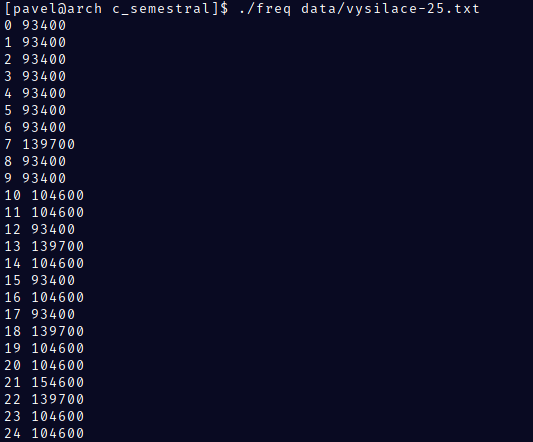
\includegraphics{img/success.png}
        \caption{Příklad správného spuštění aplikace s výsledkem}
        \label{img:success}
\end{figure}
%
Pokud není zadán argument, nebo program narazí na chybu a je neúspěšně ukončen
vypíše chybové hlášení. Příklad spuštění bez parametru viz Obrázek 
\ref{img:fail}
	%
\begin{figure}[H]
        \centering
        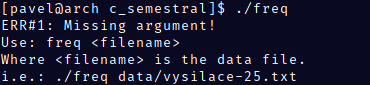
\includegraphics{img/failure.png}
        \caption{Příklad spuštění bez parametrů}
        \label{img:fail}
\end{figure}
%
\subsection{Popis chybových stavů}
Tato sekce obsahuje popis chybových stavů, které program ošetřuje a informuje
o nich.
%
\begin{table}[H]
        \begin{tabular}{|l|p{6.35cm}|}
                \hline
                \bf Chybové hlášení & \bf Popis chybového stavu \\
                \hline
                ERR\#1: Missing argument! & Programu nebyl předán očekávaný
		argument.\\
		\hline
                ERR\#2: Out of memory! & Programu se nepodařilo alokovat
		paměť.\\
                \hline
                ERR\#3: Non-existent solution! & Nelze nalézt řešení použitým
		alogritmem.\\
                \hline
                ERR\#4: Failed to open file! & Nepodařilo se otevřít soubor.\\
                \hline
                ERR\#5: Too many arguments! & Příliš mnoho argumentů, očekáván
		jeden.\\
                \hline
        \end{tabular}
        \caption{Tabulka chybových stavů}
        \label{tab:err}
\end{table}
%
% Závěr
%
\section{Závěr}
\end{document}
